\chapter{Grafteori}

Dette kapitel har til formål at beskrive og redegøre for forskellige grafer og de vigtigste elementer i grafteori. 
Grafer kan bruges til mange ting, blandt andet kortlægning af veje i en by, kloaksystemer og forskellige kredsløb.
En simpel graf defineres formel i definition \ref{def_simpel_graf}:


\begin{defn}
En graf $G = (V, E)$ består af $V$, et antal knuder, og E, et antal kanter hvorom der gælder at $V, E \neq \emptyset$
Hver kant har enten en eller to knuder, som den er forbundet til, som er dens endepunkter.
En kant siges at forbinde dens endepunkter. Denne konstruktion er en \it{simpel graf}.
\label{def_simpel_graf}
\end{defn}


\noindent En kant repræsenteres ved en linje mellem to knuder, og knuder repræsenteres ved et punkt. Har grafen enten et uendeligt antal knuder eller kanter, eller begge dele, er der tale om en \textit{uendelig graf}. Ellers betegnes grafen som en \textit{endelig graf}.


\begin{figure}[h]
\centering
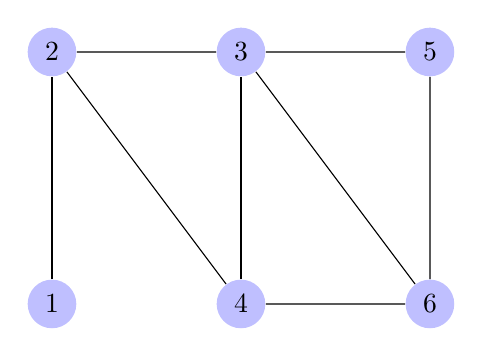
\begin{tikzpicture}
[scale=.8,auto=left,every node/.style={circle,fill=blue!25}]
  \node (n6) at (3,2) {1};
  \node (n4) at (3,6)  {2};
  \node (n5) at (6,2)  {4};
  \node (n1) at (6,6) {3};
  \node (n2) at (9,2)  {6};
  \node (n3) at (9,6)  {5};
  \foreach \from/\to in {n6/n4,n4/n5,n5/n1,n1/n2,n2/n5,n2/n3,n3/n1,n1/n4}
    \draw (\from) -- (\to);
\end{tikzpicture}
\caption{Et eksempel på en simpel, endelig graf} \label{simpel_graf}
\end{figure}


\noindent I figur \ref{simpel_graf} er skitseret en simpel graf med $6$ knuder og $8$ forbindende kanter. \\
Det kan imidlertid være nødendigt at give kanterne retning, for at indikere, hvilken retning forbindelsen mellem to punkter har. I grafer over eksempelvis trafikale netværk, kan det være nødvendigt at indikere, i hvilken retning, trafikken kører eller at angive ensrettede strækninger. Til disse formål vil en simpel graf være utilstrækkelig idet kanterne deri netop ingen bestemt retning har. Derfor anledes definition \ref{def_retn_graf} 
af en \textit{retningsbestemt graf}:

\begin{defn}
En retningsbestemt graf $G = (V, E)$ består af et antal knuder, $V$, og et antal \textit{retningsbestemte} kanter hvorom der gælder, at $V, E \neq \emptyset$.\\
En retningsbestemt kant $(u,v)$ forbinder et knudepar, så at kanten starter i $u$ og ender i $v$.
\label{def_retn_graf}
\end{defn} 

\noindent Denne definition (\ref{def_retn_graf}) tillader ydermere muligheden for, at et knudepar kan forbindes af indtil flere retningsbestemte kanter. Findes dette i grafen, kaldes den en \textit{retningsbestemt multigraf}. I det tilfælde, at alle knudepar kun forbindes af netop én retningsbestemt kant er grafen en \textit{simpel retningsbestemt graf}.

